\documentclass[00_complete]{subfiles}

%\documentclass[12pt]{report}
\usepackage[utf8]{inputenc}
\usepackage{amsmath,amssymb,amsthm,gensymb,parskip,graphicx,footmisc,csquotes,enumerate,datetime2}
\usepackage[]{libertinus}
\usepackage[breaklinks]{hyperref}
\hypersetup{
  pdfauthor={Moshe Krumbein},
  colorlinks=true,
  linkcolor={black},
  filecolor={black},
  citecolor={black}, %blue
  urlcolor={black}, %blue
}
\usepackage[top=30mm,bottom=30mm,left=30mm,right=30mm]{geometry}
%\setlength{\emergencystretch}{2em} % prevent overfull lines
\providecommand{\tightlist}{%
\setlength{\itemsep}{0pt}\setlength{\parskip}{0pt}}

\renewcommand\qedsymbol{$\blacksquare$}

\theoremstyle{definition}
\newtheorem*{definition}{Definition}
\newtheorem*{theorem}{Theorem}
\newtheorem*{axiom}{Axiom}
\newtheorem*{lemma}{Lemma}

\theoremstyle{remark}
\newtheorem*{note}{Note}
\newtheorem*{symbols}{Symbol}
\newtheorem{example}{Example}[section]
\newtheorem*{claim}{Claim}
\newtheorem*{conclusion}{Conclusion}
\newtheorem*{reminder}{Reminder}

\usepackage{fancyhdr}
\usepackage[italicdiff]{physics}
\MakeOuterQuote{"}

\renewcommand{\chaptermark}[1]{\markboth{#1}{}}

\pagestyle{fancy}

\setlength{\headheight}{14.5pt}
\addtolength{\topmargin}{-2.5pt}

\fancyhf{}
\rhead{Moshe Krumbein}
\lhead{\chaptermark}
\cfoot{\thepage}
\fancyhead[R]{\chaptername~\thechapter}
\fancyhead[L]{\mbox{\leftmark}}

\usepackage[Rejne]{fncychap}
\usepackage{titling}

\makeatletter
\renewcommand{\@chapapp}{\vspace*{-100pt}\huge\thetitle}
\makeatother

\makeatletter
\newcommand{\subtitle}[1]{%
  {\center\vspace*{-60pt}%
  \linespread{1.1}\Large\scshape#1%
  \par\nobreak\vspace*{35pt}}
}
\makeatother

\newcommand{\Chapter}[2]{
    \def\n{#2}
    \setcounter{chapter}{\the\numexpr\n-1}
    \chapter{#1}
    \subtitle{\theauthor~- \thedate}
}

\DeclareMathOperator{\Ima}{Im}
\DeclareMathOperator{\Id}{Id}
\DeclareMathOperator{\cis}{cis}

\newcommand{\Mod}[1]{\ (\mathrm{mod}\ #1)}
\newcommand{\st}[0]{\;\mathrm{s.t.}\;}


\title{Mathematical Methods}
\author{Moshe Krumbein}
\date{Fall 2021}

\begin{document}
\Chapter{Vector Functions
(\texorpdfstring{$\mathbb{R}\to\mathbb{R}^{\lowercase{n}}$}{R to Rn})}{9}

\section{Introduction}

\begin{definition}[Vector Function]
    $$f: \mathbb{R} \to \mathbb{R}^n \implies f(t) = \begin{pmatrix}
        f_1(t) \\f_2(t)\\ \vdots \\ f_n(t)
    \end{pmatrix}$$
When drawing these functions, instead of drawing the \emph{graph}, we draw the
\emph{image} of the function.
\begin{example}
    $$f: \mathbb{R} \to \mathbb{R}^2 \implies f(t) = \begin{pmatrix}
        \cos t \\ \sin t
    \end{pmatrix}$$
    The \emph{image} of this function is the unit circle.
\end{example}
\end{definition}
\section{Derivative of a Vector Function}
\begin{definition}[Derivative of a Vector Function]
    $$
    \begin{gathered}
        \dv{t}\begin{pmatrix}
            f_1(t)\\ \vdots \\ f_n(t)
        \end{pmatrix} = \begin{pmatrix}
            f_1'(t) \\ \vdots \\ f_n'(t)
        \end{pmatrix} = \dot f(t) = \underline r(t)
    \end{gathered}
    $$
\end{definition}
\begin{definition}[Linear Approximation]
    $$f(t + \Delta t) = f(t) + \dot f(t)\Delta t$$
\end{definition}
\subsection{Characteristics}
\begin{gather}
    \dv{t}(\underline r \cdot \underline w) = \dot{\underline r} \cdot
    \underline w + \underline r \cdot \dot{\underline w} \\
    \dv{t}(\underline r \land \underline w) = \dot{\underline r} \land
    \underline w + \underline r \land \dot{\underline w} \\
    \dv{t}[\underline r, \underline w, \underline u] = [\dot{\underline r},
    \underline w, \underline u] + [\underline r, \dot{\underline w}, \underline
    u] + [\underline r, \underline w, \dot{\underline u}]
\end{gather}
\begin{example}
    $$\dv{t}(\underline r \cdot \underline r) = 2\underline r \cdot
    \dot{\underline r}$$
\end{example}
\section{Integral of a Vector Function}
\begin{definition}[Integral of a Vector Function]
    $$\int \underline f(t)\dd{t} = \begin{pmatrix}
        \int f_1 \\ \vdots \\ \int f_n
    \end{pmatrix}$$
\end{definition}
\section{Complex Functions}
$$f: \mathbb{R} \to \mathbb{C}$$
We can look at this function as if it was $f: \mathbb{R} \to \mathbb{R}^2$
\begin{example}
\begin{gather*}
    f(t)=e^{i\omega t} = \cos(\omega t) + i\sin(\omega t) \\
    \dot f(t) = - \omega \sin(\omega t) + i \omega \cos(\omega t) \\
    =i\omega(\cos(\omega t) + i\sin(\omega t)) = i \omega e^{i \omega t}
\end{gather*}
\end{example}
\section{Length of a Curve}
Given curve $\underline r(t)$, its velocity vector is $\dot{\underline r}(t)$.

Its scalar velocity is defined as $\|\dot{\underline r}(t)\|$, or simply $\dot r(t)$.

The length of the curve from $\underline r(a)$ to $\underline r(b)$ is defined
as:
$$\int_{a}^{b} \|\dot{\underline r}(t)\|\dd{t}$$
\begin{example}
    $$
        \underline r(t)=\begin{pmatrix}
            \cos t \\\sin t
        \end{pmatrix}_{0 \leq t \leq 2\pi}
    $$
    The length of the curve is:
    $$\int_{0}^{2\pi}\|\dot{\underline r}(t)\|\dd{t} =
    \int_{0}^{2\pi}\underbrace{\left\|\begin{pmatrix}
        -\sin t \\ \cos t
    \end{pmatrix}\right\|}_{1}\dd{t} = \int_{0}^{2\pi}\dd{t} = 2 \pi$$
\end{example}
\begin{example}
    \label{screw}
    $$\underline r(t) = \begin{pmatrix}
        t \cos t \\ t \sin t \\ t
    \end{pmatrix}$$
    \begin{figure}[ht]
        \centering
    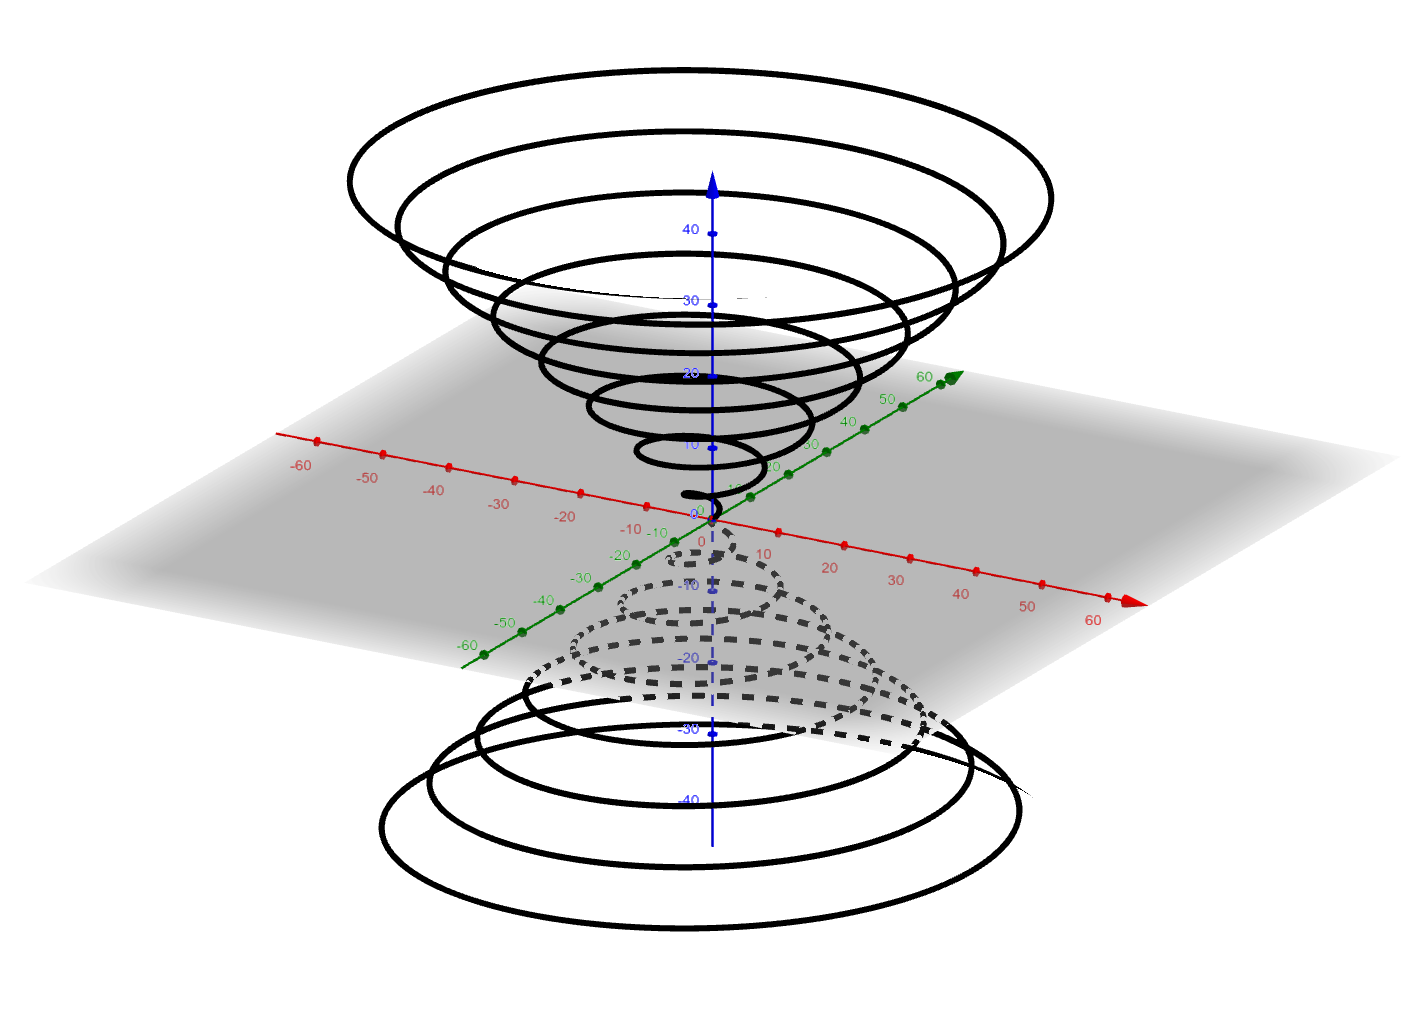
\includegraphics[width=0.5\textwidth]{corkscrew}
    \caption{Graph of $\underline r(t)$ in Example \ref{screw}}
    \end{figure}
    \begin{gather*}
    \dot{\underline r}(t) = \begin{pmatrix}
        \cos t - t\sin t \\ \sin t + t \cos t \\ 1
    \end{pmatrix} \\
    \|\dot{\underline r}(t)\| = \sqrt{t^2+2}
    \end{gather*}
    The length of the curve:
    $$\int_{a}^{b}\sqrt{t^2+2}\dd{t}$$
\end{example}
\end{document}
